\section{Lighthouses: Treating Places as People}

% \subsection{Limitations of Person-Person EN}

Despite their promise, there remains significant concern around the efficacy of privacy-preserving contact tracing and exposure notification protocols.
For one thing, not everyone has access to a mobile phone, and many that do may be unwilling to participate (even Singapore only achieved 20\% adoption\cite{traceTogether20pct}). 
This is a serious concern as the probability of a successful detection grows quadratically with participation~\cite{pact}. 
Of course, manual contact tracing does not have this issue and remains the gold standard. 
Will these two techniques exist in isolation or will they interact synergistically? 
Finally, bluetooth contact detection is limited in range and time; it cannot detect many important forms of transmission like surfaces or HVAC systems\cite{hvacTransmission}.

\subsection{Treating Places as People}
There is a simple extension to mobile contact tracing that can help address these issues. 
The idea is rooted in centuries old maritime signaling. To navigate at night, ships use signal lights, much like our Bluetooth beacons, to identify and safely navigate around nearby ships. 
However, to safely sail at night, ships also rely on lighthouses, strategically placed beacons, to identify and safely navigate around key landmarks. 
It is this second form of beacon, the lighthouse, that is needed to address several of the key limitations in privacy-sensitive mobile contact tracing.

\subsection{What is an Exposure Notification Lighthouse?}
A privacy-sensitive exposure notification lighthouse is a device (e.g., a mobile phone or even a smart sticker) deployed in a public space following the same privacy sensitive mechanisms as individuals. Figure \ref{fig:lighthouseDevices} gives a few examples of what lighthouses could look like.
Much like the maritime lighthouse, contact tracing lighthouses can be used to inform others of potential exposures associated with public spaces discovered through manual contact tracing. 
A contact tracing lighthouse can also log passing beacons to inform owners and public health authorities of exposure risks. However, because the lighthouse follows the same privacy-sensitive protocols as individuals, it retains all of the privacy guarantees of the existing protocols. Moreover, by installing contact tracing lighthouses in participating public spaces ranging from stores and restaurants to schools and buses, we introduce a privacy sensitive mechanism to bridge manual contact tracing with mobile contact tracing. Such a bridge gives public health authorities the ability to gain visibility into the spread of disease while preserving individual privacy.

\begin{figure}[h]
    \centering
    \begin{subfigure}[t]{0.3\textwidth}
        \centering
        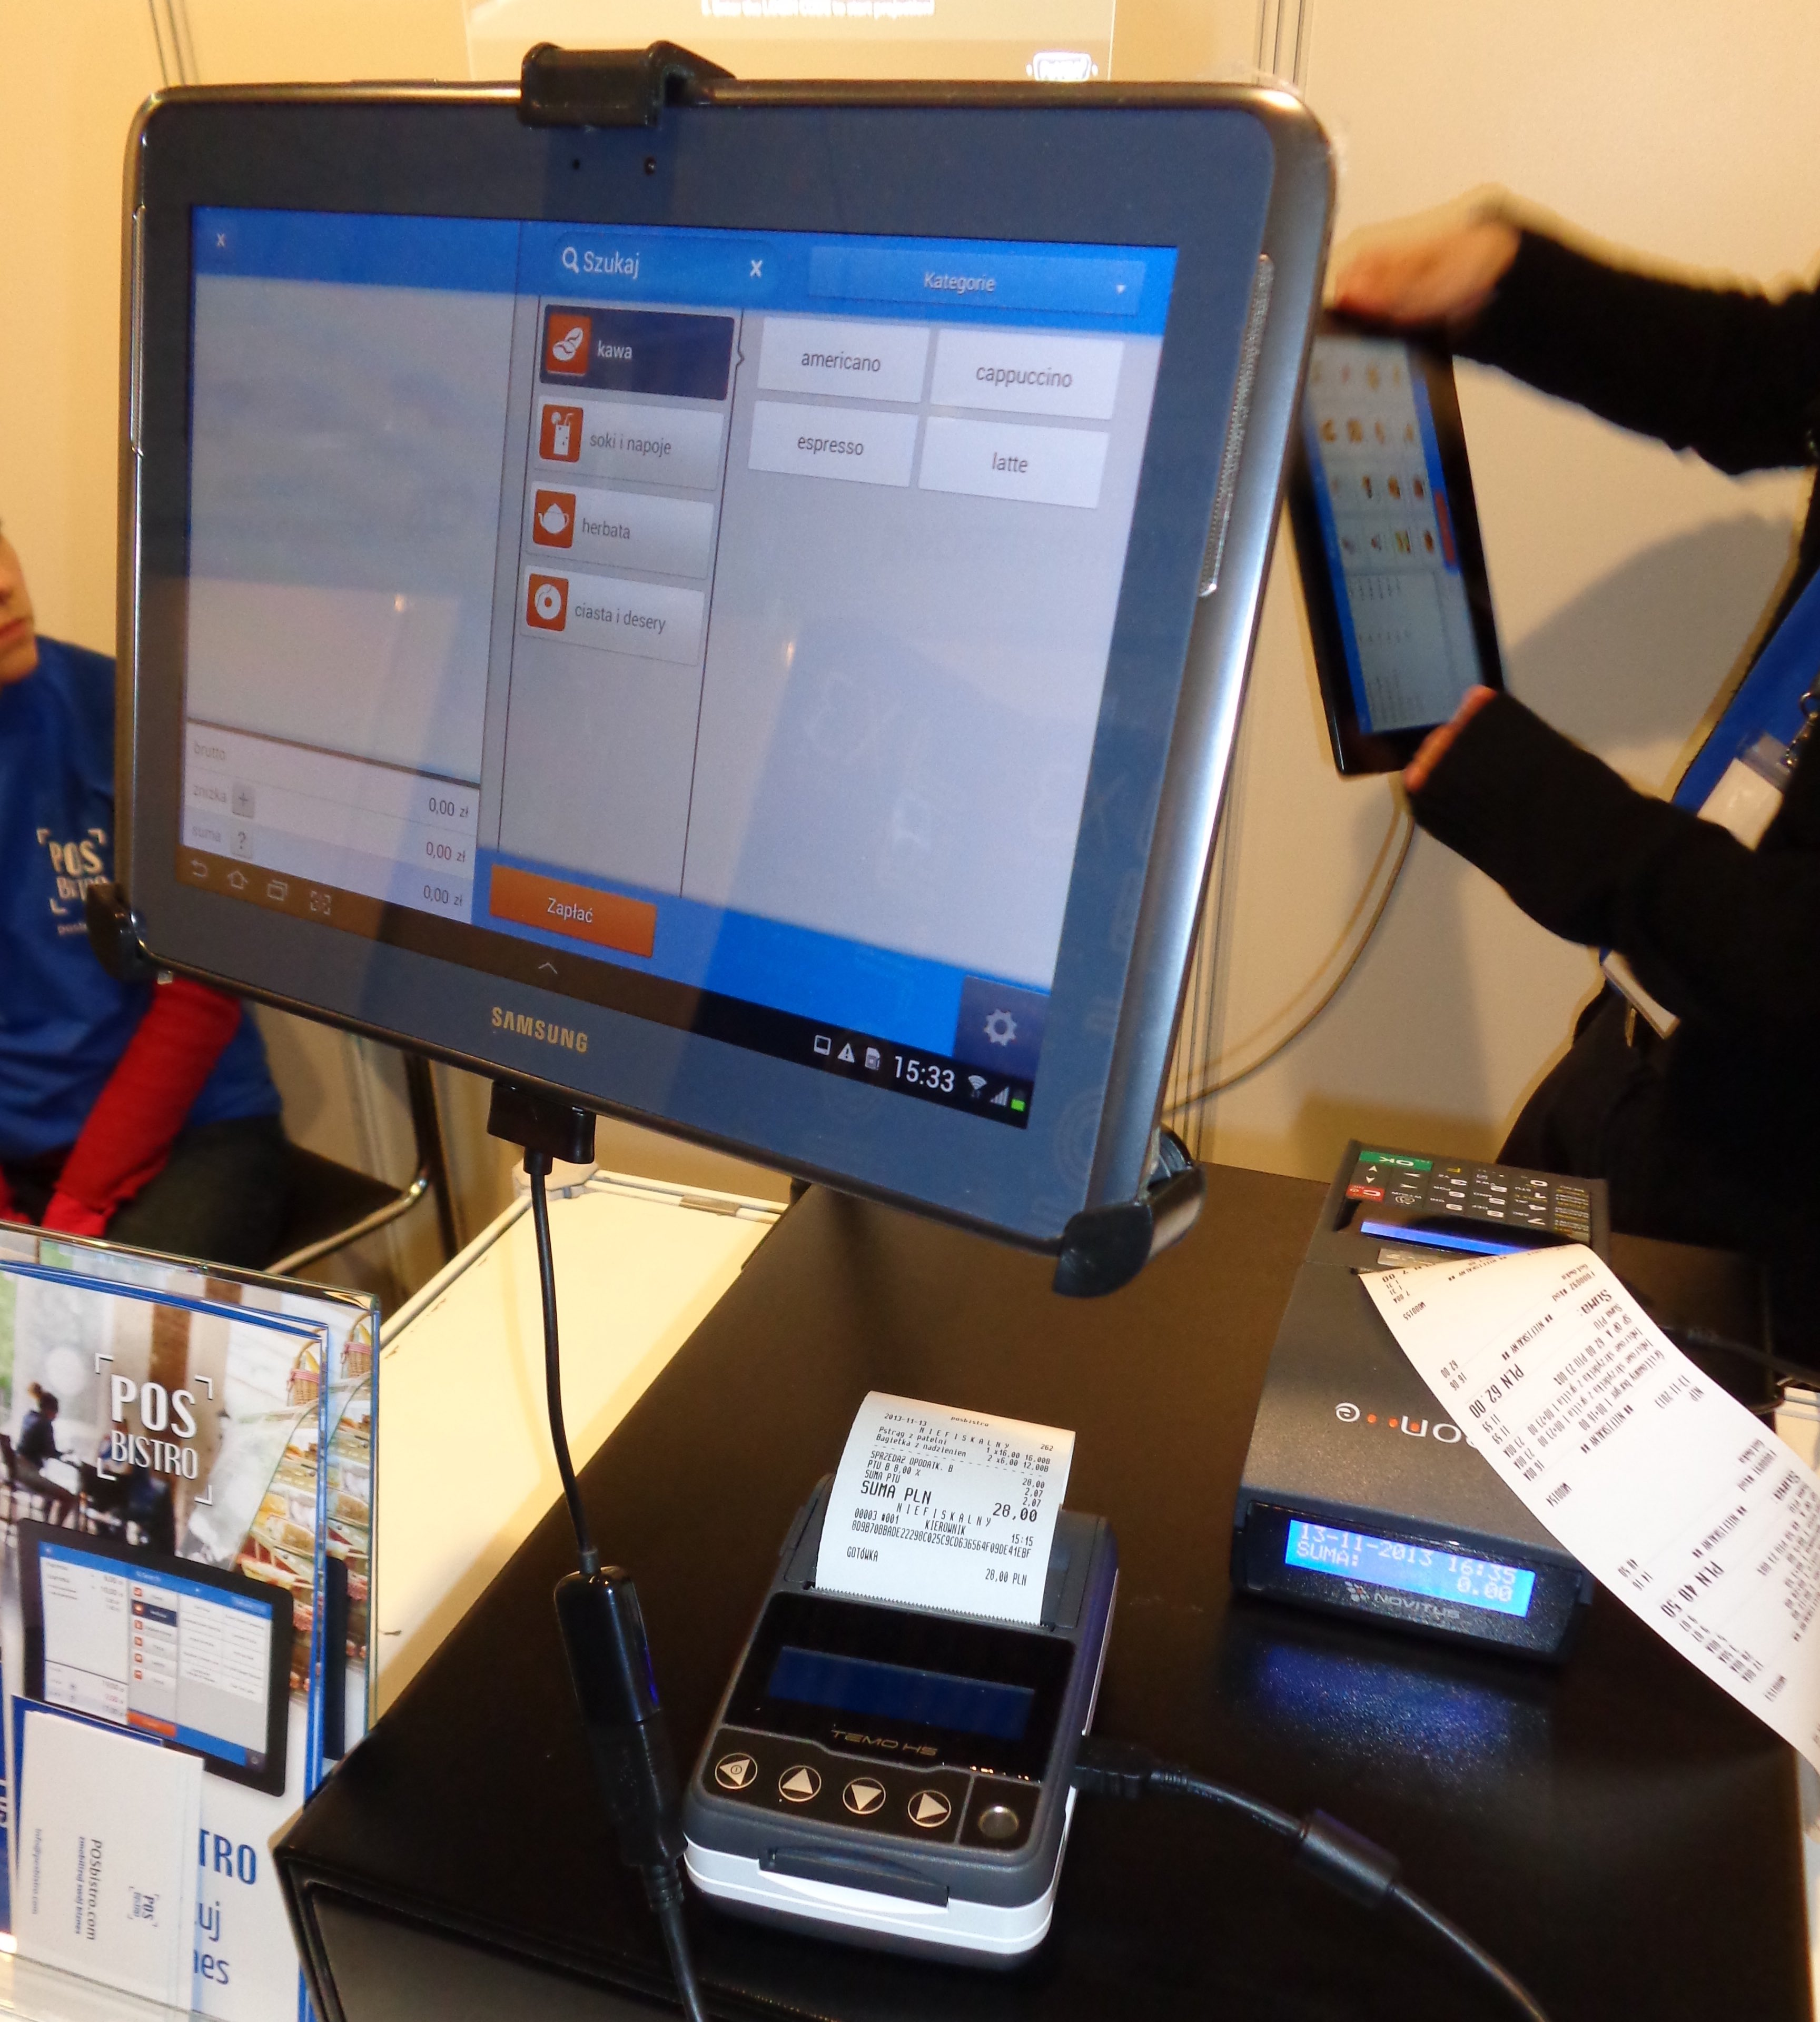
\includegraphics[width=0.9\textwidth]{figs/POS.jpg}
        \caption{\textbf{Existing Devices:} Easily deployed immediately but expensive to deploy to new places. They can also be unreliable when unattended.}
        \footnotetext{wikimedia commons © Travelarz CC-ASA 3.0}
    \end{subfigure}
    ~
    \begin{subfigure}[t]{0.3\textwidth}
        \centering
        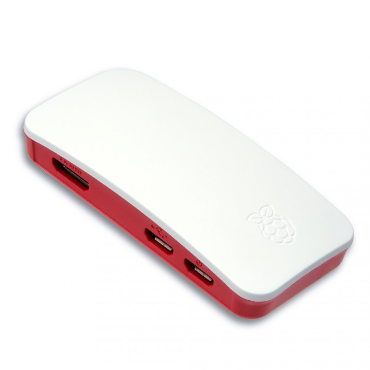
\includegraphics[width=0.9\textwidth]{figs/RaspberryPi.png}
        \caption{\textbf{Dedicated Devices:} Cheap and reliable. They will require new development and can be tricky to place correctly.}
    \end{subfigure}
    ~
    \begin{subfigure}[t]{0.3\textwidth}
        \centering
        
\includegraphics[width=0.9\textwidth]{figs/physicalRPI.pdf}
        \caption{\textbf{No Device:} Allows those without the app or even a mobile device to participate. They may be easier to re-identify and require manual effort from users to check.}
    \end{subfigure}
    \caption{Lighthouses can be deployed using a number of different devices with varying trade-offs. Each of these examples is feasible to deploy in the near future.}
    \label{fig:lighthouseDevices}
\end{figure}

\subsection{What Do We Get From Lighthouses?}
Figure \ref{fig:lighthouseExample} walks through an example of how lighthouses could work in a typical case. Let's explore some of these benefits in more detail.
\begin{figure}
    \centering
    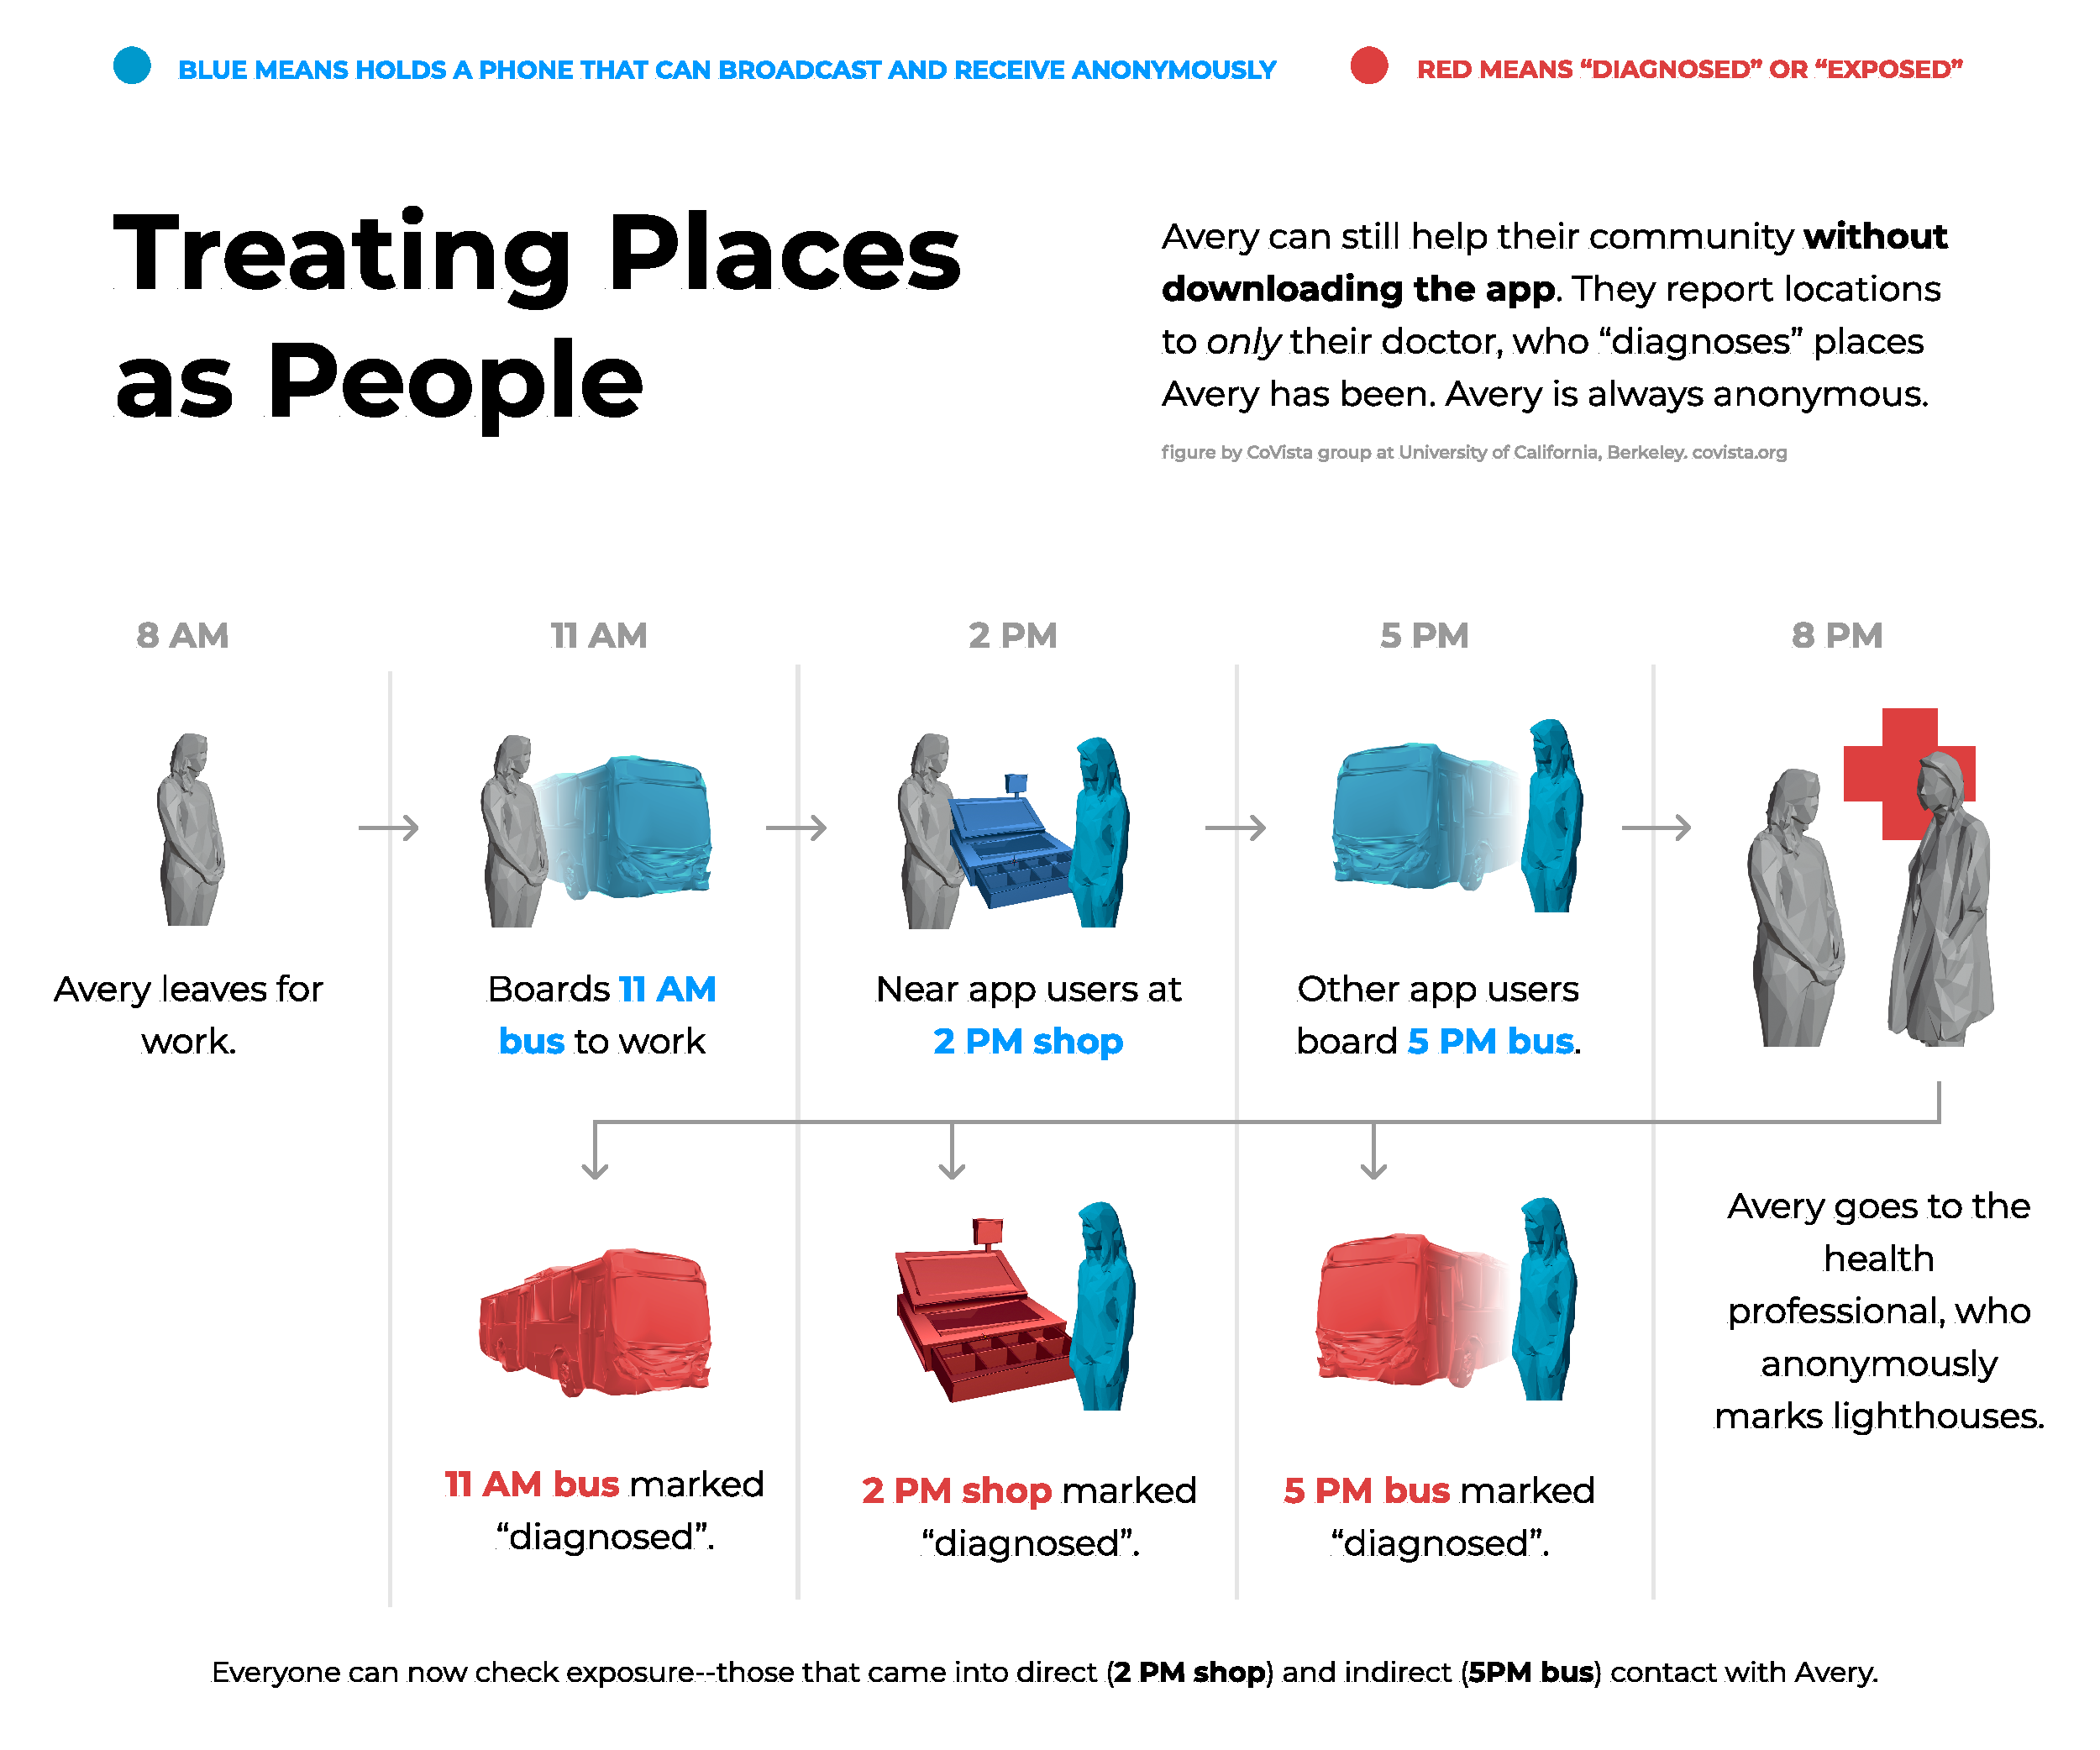
\includegraphics[width=\textwidth]{figs/how_lighthouse_works.pdf}
    \caption{An example scenario of an affected individual (Avery) and a stranger (Bernie) that may have been exposed. Even if Avery is not an app user, the doctor can still notify the shop and bus of their exposure; lighthouses \textbf{connect manual and mobile contact tracing}. Lighthouses \textbf{bridge place and mobile} by allowing the bus and shop to notice their exposure and mark themselves as exposed, even if Avery did not remember visiting them. They also \textbf{enabled less direct forms of exposure} by notifying Bernie of their potential exposure, even though they were not on the bus at the same time as Avery. Finally, lighthouses offer places benefits \textbf{beyond the standard mobile contact tracing}. They can now track how often they are exposed, at what times, and even in which section within them (if they have multiple lighthouses installed).}
    \label{fig:lighthouseExample}
\end{figure}

\shankari{In Fig.~\ref{fig:lighthouseExample}, Avery needs to be diagnosed COVID+ when they go to the health professional. Small change but it needs to happen in Figma}

\shankari{We have generally been using gender-neutral names - Avery and Jordan. Bernie reads as male to me. Use Jordan again?}

\subsubsection{Bridging Place and Mobile}
The contact tracing lighthouse empowers stewards of public spaces (e.g., shop owners, school administrators) to collaborate with public health authorities to help mitigate the spread of disease without jeopardizing the privacy of patrons or the reputation of the public spaces. When an individual is tested and confirmed, the manual contact tracing interview process begins. One of the first questions asked is “Can you recall where you have been that might have exposed others?”. A place, unlike an individual, has a large set of explicit relationships with its institutional environment - business license, health department approvals, chamber of commerce, etc. The interview process routinely seeks to gather information about places. But often there is little the place can do to help. With its lighthouse, it has a very simple way to provide assistance without undue impact on its reputation. Just like a person, it can check its own potential exposures. And, like a person, it can anonymously publish its own random numbers as COVID positive so that people can use them for detecting their exposure risk. This is especially useful if the individual who tested positive was not using an app that broadcasts their own sequence of random numbers. Unlike a person’s phone, stationary lighthouses can be carefully positioned to avoid issues like weak or unreliable broadcast that mobile phones can face. Finally, the public place may also take other measures in assisting its local health authority in detecting hot spots, such as informing them of the exposure risk that it observes.

\subsubsection{Indirect Transmission}
The lighthouse can be used to address forms of indirect transmission that are not captured in the existing privacy-sensitive mobile contact tracing efforts. If a COVID-positive individual enters a bus and touches or sneezes on several surfaces they could potentially infect others over the next several hours, long after they have left the bus. Air conditioning systems have also been implicated in spreading the virus over large distances~\cite{hvacTransmission}. Existing wireless protocols will fail to capture these forms of transmission since they rely on close, contemporaneous radio proximity with the positive individual. However, with the introduction of the lighthouse, the bus or restaurant can automatically determine that it was exposed and choose to anonymously publish its own random number sequence.

\subsubsection{Beyond Mobile Contact Tracing}
Finally, the lighthouse can also extend the privacy-sensitive mobile contact tracing protocol beyond the smartphone. Places provide channels of communication to individuals that complement smartphones. Simple lighthouse codes might be included on printed receipts or handed to customers. A person without contact tracing on their phone might use such code to manually perform the exposure checks that are automated by the apps. For example, they could enter such codes that they have received into a public website to determine their exposure risk.

\subsection{Lighthouse Privacy}
There are legitimate privacy interests for places, as there are for people. 
Businesses may fear irrational boycotts or loss of reputation, and there are risks of perpetuating prejudice or stigma against neighborhoods or ethnic groups (already a growing problem \cite{asianDiscrimination}). The good news is that lighthouses inherit the privacy protecting characteristics of the AGEN protocol. In their simplest form, they are phones running ordinary apps, different only because they live in a fixed place rather than in purse or pocket.

Lighthouses can complement manual contact tracing by offering greater confidentiality in situations where people cross paths in stigmatized locations. For example, investigators following up on a recent case cluster associated with nightclubs in Korea catering to the LGBTQ community have struggled to contact attendees who are afraid of being “outed” or facing discrimination \cite{koreaClub}. Lighthouses can fill such gaps without requiring or relying on anyone, even an affected person, to disclose their location history.

A potential concern about lighthouses is that internal state, if combined and aggregated, could be used to undermine some of the privacy guarantees of AGEN. 
Indeed, with a sufficiently large deployment of lighthouses and centralized collection of recieved RPIs, it would be possible to resolve the locations of all the COVID positive individuals.
We therefore stress that each lighthouse must follow the existing decentralized protocol for risk assessment in which only risk is aggregated and not the underlying RPIs.  

To address some of these security concerns, it is possible to deploy \textbf{transmit only} (passive) lighthouses which could be used to anonymously notify others of exposure without listening for RPIs.  
This eliminates the risk of resolving COVID positive individuals locations but also limits visibility into where the disease is spreading.  


